\chapter{Implementation}
The implementation is divided into several modules: \textit{core} (code for computing different equilibria), \textit{web} (a backend engine that allows to play games and stores the results in a database), \textit{console} (a console client for the web API), \textit{structures} (common structures for \textit{web} and \textit{console}), and \textit{analysis} (Spark code to analyze large datasets of games).
Each module is described in a separate section below.

There are several services ready to be used via Docker Compose, and can simply be run without the need of installing any additional software:
\textit{web} (the web API server), \textit{postgres} (a PostgreSQL database; is started automatically when running \textit{web}), \textit{console} (the console interface), \textit{analysis} (Apache Spark with commands from the \textit{analysis} module made available), and \textit{sbt} (the building tool; can be used to compile modules and to run tests).

\section{Core module}
While the core module does not contain much code, it is the heart of this project.
It defines the following entities:
\begin{itemize}
	\item \textsc{Game}: a case class that represents a game in normal form for two players.
	\item \textsc{BestResponse}: a trait that describes a best response, given a game and the opponent's strategy.
	It is implemented by the following objects:
	\begin{itemize}
		\item \textsc{NashianBestResponse}
		\item \textsc{PerfectlyTransparentBestResponse}
	\end{itemize}
	\item \textsc{GameGenerator}: an object for generating random games.
\end{itemize}

\section{Web module}
\label{sec:impl-web-module}
The web module is a web server that provides a REST API for playing games in normal form against a computer.
Every time a game is played, the result is stored in a PostgreSQL database (see \autoref{fig:db-schema}).
The API exposes the following endpoints:
\begin{itemize}
	\item \textsc{NewUser}: Creates a new user and returns the user's ID.
	\item \textsc{NewGame}: Starts a new game; returns the game matrix and ID.
	\item \textsc{Play}: For a game with given ID, accepts the human-player's (row) strategy, and returns the computer's (column) strategy.
	\item \textsc{Stats}: Returns statistics for a user with given ID: number of games played and the average payoff.
\end{itemize}

Play Framework is used to implement the server.
For communicating with the database, we use Slick library.

\begin{figure}
	\hspace{-1cm}
	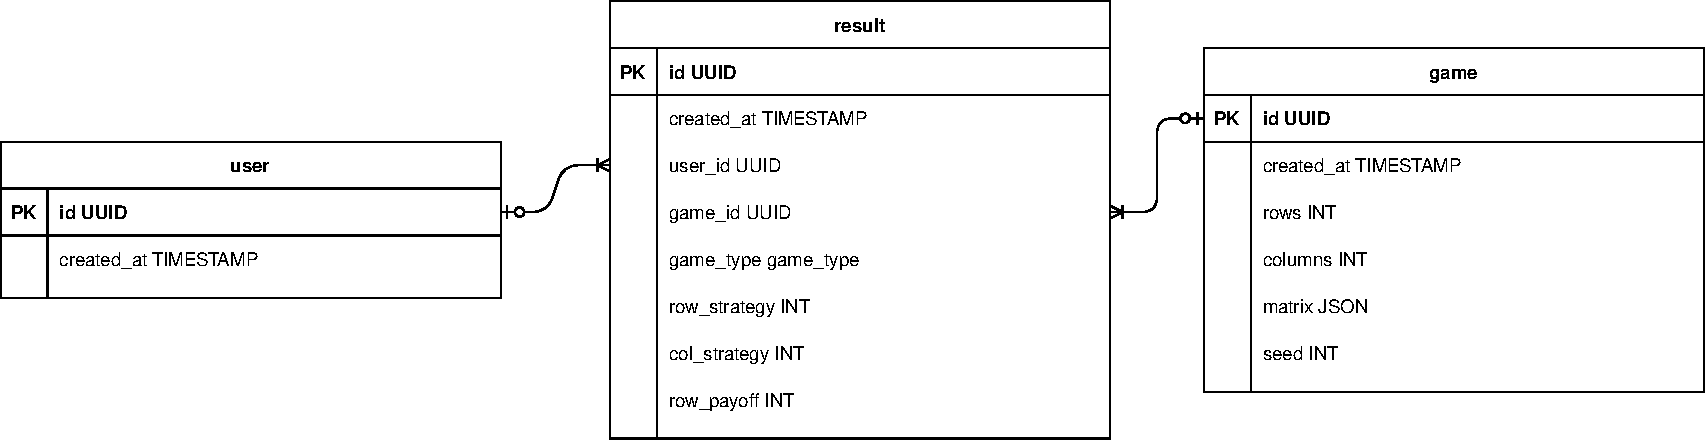
\includegraphics[width=14cm]{fig/schema.pdf}
	\caption{The database schema.}
	\label{fig:db-schema}
\end{figure}

\section{Console module}
The console module is a sample client for the REST API described in \autoref{sec:impl-web-module}.
It allows the user to play a series of games of chosen dimensions.
For each game, the game matrix is displayed and the user is asked to choose a strategy.
After choosing a strategy, the computer's strategy and the resulting payoff is displayed.
Then, the user is asked whether she wants to play another game.
At the end, statistics over all games are displayed.

\begin{figure}
	\centering
	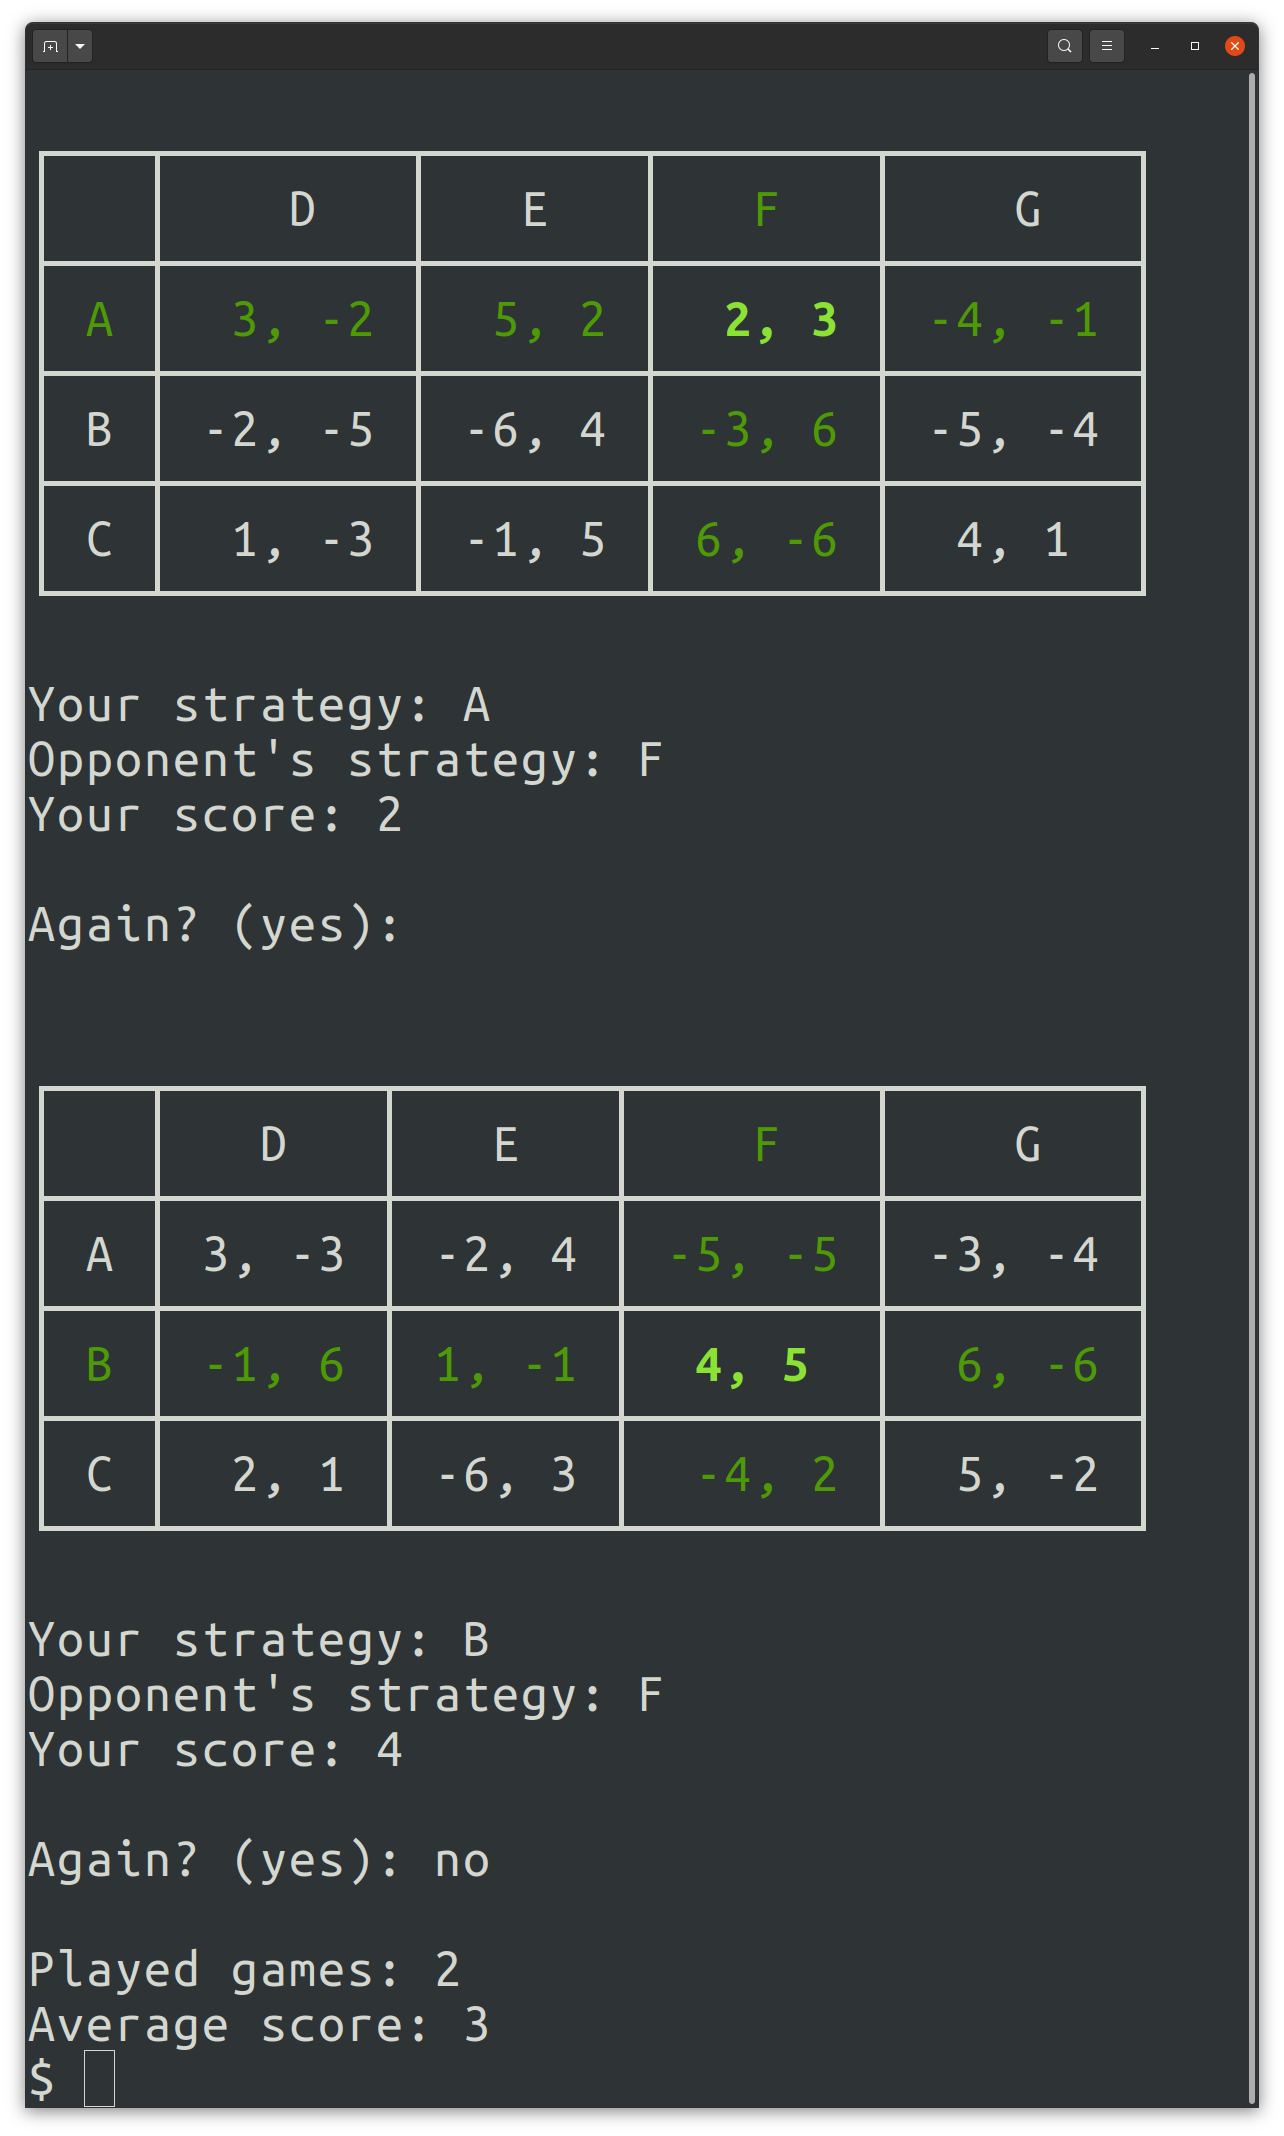
\includegraphics[width=12cm]{fig/console.png}
	\caption{The console interface.}
	\label{fig:console-screen}
\end{figure}

\section{Analysis module}
The analysis module is used for computing statistics about large datasets of games using Apache Spark.
It loads the datasests and computes the PTBPE, PTBRE, individually rational and minimax rationalizable strategy profiles, and stores them as a new dataset.
Searching through this dataset was useful to find counterexamples and form conjectures about inclusions of these equilibiria (see \autoref{chap:game-theory}).
